\section{Introduction}
The accuracy of the statistical estimation depends on 
not only the way of building probability models
but also both the quality and the quantity of the samples.
From this viewpoint, one drawback of the current EAPM
is the absence of a population maintenance mechanism, 
where a part of the historical samples are reused,
whereas 
Genetic Algorithms (GAs) \cite{goldberg:ga} have used ones for a long time.
In GAs, various population maintenance techniques \cite{shimodaila:nitching} 
were proposed and
they are intuitively combined with EAPM in some works, 
for example, Bayesian optimization algorithms (BOAs) \cite{pelikan:99boa}, 
hierarchical Bayesian optimization algorithm (hBOA),
\cite{pelikan:escaping,pelikan:robust,pelikan:dependency}, and iterated density estimation evolutionary
algorithm (IDEA) \cite{bosman:idea,bosman:idea2}.
Indeed, they break the mathematical structure of EAPM;
EAPM are regarded as methods building probability models
approximating the target distributions, 
which explicitly represent the distributions of promising solutions.
In the heuristic population mechanisms,
the distribution of the population (i.e., the selected historical samples) is normally unknown
and the built probability model is no longer related 
to the target distributions.


This chapter proposes a novel population maintenance method,
resampling population model (RPM)
that maintains a part of the historical samples such that
they seem to follow the target distribution by weighting generated samples.
This implies that the probability model 
of the population approximates the target distribution.
To control the size of the population, resampling is employed.
The aim of this chapter is to investigate the effectiveness of RPM
through experimental comparisons with conventional methods.



\section{Resampling Population Model (RPM)}
The primary objective of RPM is
to extend the calculation of (\ref{eapm-ml})
to using not only the currently generated samples 
but also the population, that is, a part of the historical samples.
This implies that RPM is an extension of the EAPM.
If all the historical samples in all previous iterations are
completely maintained,
according to importance sampling, the empirical log-likelihood is given by
\begin{equation}
\label{all_history}
 L\simeq\frac{1}{|X|}\sum_{X} \frac{q_{t+1}(x)}{\sum_{i \leq  t} \alpha_i p_i(x)} \log p_{t+1}(x),
\end{equation}
where $X$ is a set of all the historical samples,
which are generated from all the built probability models
and $\alpha_i$ is the ratio of the number of the samples generated from
$p_i(x)$.
\footnote{
If all the historical samples from the $k$ previous iterations are
completely maintained,
according to importance sampling, the empirical log-likelihood is given by
\begin{equation}
 L\simeq\frac{1}{|X|}\sum_{X} \frac{q_{t+1}(x)}{\sum_{t-k\leq i \leq  t} \alpha_i p_i(x)} \log p_{t+1}(x),
\end{equation}
where $X$ is a set of all the historical samples,
which are generated from all the built probability models
and $\alpha_i$ is the ratio of the number of the samples generated from
$p_i(x)$.
This method may be practical, but we cannot control which samples are
maintained in this way.
Therefore, this is out of scope.
}
However, the secondary objective of RPM is to control the size of
the population.
In other words, 
important samples are selected and the remains are discarded.

In the following,
first, the key calculation technique for
weighting samples is described in Section \ref{sec-gis}.
Section \ref{sec-rpm-algorithm} describes how RPM
maintains the population based on this technique. 
Finally, Section \ref{sec-rpm-detail} describes the details for implementation.

\subsection{Weighted Samples Approximating Distribution}
\label{sec-gis}
If a sample set $X$ whose samples are generated from $p(x)$ are given
and their weights are defined by 
\begin{equation}
 w_i \propto \frac{q(x_i)}{p(x_i)} \ \mathrm{for} \ x_i \in X, \label{def-weight}
\end{equation}
then
we define a probability distribution $\hat q(x)$ as follows:
\begin{equation}
 \hat q(x)= \frac{1}{\sum_{X} w_i}\sum_{x_j \in X} w_i \delta(x-x_i),
\label{particle-distribution}
\end{equation}
where $\delta(\cdot)$ is the delta function.
The expectation of any function $f(x)$ 
with respect to $\hat q(x)$ is exactly given by
\begin{equation}
 \int \hat q(x) f(x) dx = \frac{1}{\sum_X w_j}\sum_X w_i f(x_i).\label{pop-nis}
\end{equation}
This is equivalent to normalized importance sampling.

Let us assume $w_i=\frac{q(x_i)}{p(x_i)}$.
Then, the expectation of $\sum_X w_i$ is the number of samples in $X$,
that is, $E[\sum_X w_i]=|X|$.
Especially,
if $\sum_X w_i=|X|$, (\ref{pop-nis}) reduces to normal importance sampling.
Hence, we can regard $\hat q(x)$ as
an approximation distribution of $q(x)$.
This technique is well known 
in sequential Monte Carlo methods \cite{doucet:particle}
\footnote{
RPM is based on the technique of sequential Monte Carlo methods.
Actually, the relationships between sequential Monte Carlo methods and 
Genetic Algorithms was pointed in \cite{higuchi:ga-pf}.
}.

In RPM, an additional extension is important.
This can be extended to calculate the expectation with
arbitrary $q^* (x)$ as follows:
\begin{eqnarray}
\int q^*(x) f(x) dx &=& \int q(x) \frac{q^*(x)}{q(x)} f(x)dx\\
                    &\simeq& \int \hat q(x) \frac{q^*(x)}{q(x)} dx\\
                    &=& \frac{1}{\sum_X w_j} \sum_X w_i
		     \frac{q^*(x)}{q(x)} f(x), \label{pop-gnis}\nonumber \\
\end{eqnarray}
where $w_i$ is defined by (\ref{def-weight}).
If $q(x)=q^*(x)$, (\ref{pop-gnis}) reduces to (\ref{pop-nis}).
If $q(x)=p(x)$, (\ref{pop-gnis}) reduces to normal importance sampling.
This gives an unified interpretation of normal importance sampling and
normalized importance sampling.
If the target distribution currently approximated by the
weighted samples is changed
the weights are redefined as follows:
\begin{eqnarray}
 w^*_i && \propto  w_i \frac{q^*(x_i)}{q(x_i)} \label{weight-shift} \\
 &&  \propto     
\frac{q(x)}{p(x)}
\frac{q^*(x_i)}{q(x_i)}=\frac{q^*(x_i)}{p(x)}.  \nonumber
\end{eqnarray}
The advantage of this extension is that
once the weights are determined 
we can forget how samples are generated,
that is, $p(x)$.


\subsection{Algorithm}
\label{sec-rpm-algorithm}
If the population $X_{pop}^{(t)}$,
which is supposed to be a set of unweighted samples here,
 is generated from the target
distribution,
the empirical log-likelihood can be calculated from the population and
the currently generated samples as follows:
\begin{eqnarray}
 L&=&\int r_{t}(x) \frac{q_{t+1}(x)}{r_{t}(x)}\log p_{t+1}(x)
  dx \\
&\simeq&\frac{1}{|X_m^{(t)}|}\sum_{X_m^{(t)}}
\frac{q_{t+1}(x)}{r_{t}(x)} \log p_{t+1}(x),\label{rpm-mix-is}
\end{eqnarray}
\begin{equation}
  r_{t}(x)=\alpha^{(t)} q_{t}(x) + (1-\alpha^{(t)}) p_{t}(x),
\end{equation}
\begin{equation}
\alpha^{(t)}=\frac{|X_{pop}^{(t)}|}{|X_{pop}^{(t)}|+|X_{samp}^{(t)}|},
\end{equation}
\begin{equation}
 X_m^{(t)}=X_{pop}^{(t)} \cup X_{samp}^{(t)},
\end{equation}
where 
$X_{samp}^{(t)}$ is a set of the currently generated samples,
 which follow $p_t(x)$.


To maintain the population to follow the target distribution, 
RPM weights samples according to the method described
in Section \ref{sec-gis}.
It is assumed that 
the initial population follows a uniform distribution and
the initial target distribution $q_1(x)$ is also a uniform distribution.
Thus, the initial population is defined by
\[
 X_{pop}^{(1)}=\{(1,x_i^{(1)})\}_{i=1}^{N},
\]
where each $x_i$ is generated
from a uniform distribution and 
$N$ is the number of weighted samples in the population.
The population at time $t$ is denoted by
\[
 X^{(t)}_{pop}=\{(w^{(t)}_i,x^{(t)}_i)\}_{i=1}^{N},
\]
and their weights are calculated from the previous population as the following:
Let us consider the following importance sampling:
\begin{eqnarray}
 L&\simeq&\int \hat r_{t}(x)
\frac{q_{t+1}(x)}{r_{t}(x)}\log p_{t+1}(x) dx\\
&\simeq& \frac{1}{|X_m^{(t)}|}\sum_{X_{samp}^{(t)}}\frac{q_{t+1}(x_i)}{r_{t}(x_i)}
\log p_{t+1}(x_i)\nonumber\\
&+& \frac{1}{|X_m^{(t)}|}\sum_{X_{pop}^{(t)}}w_i^{(t)}\frac{q_{t+1}(x_i)}{r_{t}(x_i)}\log
 p_{t+1}(x_i),\nonumber \\
\label{math-rpm}
\end{eqnarray}
\begin{equation}
  \hat r_{t}(x)=\alpha^{(t)} \hat q_{t}(x) + (1-\alpha^{(t)}) p_{t}(x).
\end{equation}
This is equivalent to (\ref{rpm-mix-is}) 
whose $r(x)$ is replaced with $\hat r(x)$.
In this thesis, 
$|X_{pop}^{(t)}|=\sum w_i^{(t)}$ is defined by the effective
number which is explained later, 
and $\alpha^{(t)}$ can be determined.
Let
\[
X_{samp}^{(t)}=\{(w_i^{(t)},x_i^{(t)})\} 
\]
where \mbox{$w_i^{(t)}=1$},
then (\ref{math-rpm}) can be rewritten
as 
\begin{equation}
 L \simeq \frac{1}{\sum_{X_m} w_j}\sum_{X_m^{(t)}}w_i^{t} \frac{q_{t+1}(x_i)}{r_{t}(x_i)}
\log p_{t+1}(x_i).
\label{gis-merginal-likelihood}
\end{equation}
According to (\ref{weight-shift}) and (\ref{gis-merginal-likelihood}),
the weight update rule is given by
\begin{equation}
 w_i^{t+1}=w_i^{t} \frac{q_{t+1}(x_i)}{r_{t}(x_i)}.
\label{weight-update}
\end{equation}


The secondary objective is to select important samples for
decreasing the size of the population.
The point is to prevent the accuracy of the approximation of
$\hat q(x)$ from becoming worse.
For this purpose,
RPM basically selects the samples with probabilities proportional to the
weights and this is equivalent to
sampling from $\hat q(x)$ defined by (\ref{particle-distribution}).
Since it is preferable to avoid selecting overlapping samples,
the population is represented by weighted samples.
Obviously, one appropriate method is iteratively 
selecting  samples by resampling with replacement and accumulating them
but this is not practical in terms of computational cost.
Another method is
simply selecting the highest weight samples without changing the weights.
$\hat q(x)$ can be a consistent estimator but this method
breaks the consistency. 
There is an intermediate method between the previous two methods.
that is to employs resampling (proportional to the weights) WithOut replacement (RWOR) without
changing the weights.
Note that RWOR can be quickly carried out \cite{efraimidis:rwor}.
In this chapter, RWOR is employed. 
Furthermore investigations on this topic are left as future works.


\subsubsection{Effective Number of Samples}
The population is defined by weighted samples
as $\{(w^{(t)}_i,x^{(t)}_i)\}_{i=1}^{N}$.
The size of the population cannot be defined by $\sum w_i$
because each $w_i$ is defined by a value proportional to
$\frac{q(x)}{p(x)}$.
Let us consider the normalized weight $\hat q(x_i)=\frac{1}{\sum w_j}{w_i}$.
This becomes a probability distribution and
the average probability of $\hat q(x)$
is defined by $\bar q=\exp(\int \hat q(x) \log \hat q(x)dx)$.
This can be regarded as an approximation,
where $w_i$ is given by $\bar q$ or $0$.
Under this approximation,
the number of samples with nonzero weight is given by
\begin{equation}
 \bar q^{-1}=\exp(-\int \hat q(x) \log \hat q(x)dx)
\end{equation}
and this is called the effective number.
The same idea have been introduced in \cite{shimodaira:wis-aic}.



\subsection{Numerical Calculation  Details}
\label{sec-rpm-detail}
The procedure of RPM is described as follows:
In initialization,
the initial population $X_{pop}^{(1)}$ and 
the initial set of generated samples $X_{samp}^{(1)}$ are generated
from a uniform distribution.
Thus, the target distribution $q_1(x)$
and
the initial sampler $p_1(x)$ are uniform distributions.
For generating the next population $X_{pop}^{(t+1)}$ and 
the next samples $X_{samp}^{(t+1)}$,
first, the next target distribution $q_{t+1}(x)$ is defined.
In this chapter,
target distributions are defined by partially uniform
distributions,
which are defined by (\ref{pud}), and therefore
the threshold parameter $\tilde f$ in (\ref{truncation})
is determined to define the target distribution.
%%
$\tilde f$ is selected
such that the number of samples which satisfies $q_{t+1}(x) \neq 0$,  
becomes $N'(<N)$, which is previously defined by the cutoff rate
$c=\frac{N'}{N}$, where $N$ is the number of samples 
in the current population. 
%%
To investigate RPM with using other probability distribution families
such as Boltzmann distribution for target distributions 
is carried out in Chapter \ref{chapter-ers}.

The merged set $X_m^{(t)}=X_{pop}^{(t)} \cup X_{samp}^{(t)}$
is generated.
The weights of the samples in $X_m^{(t)}$ are updated according to
(\ref{weight-update}).
(\ref{weight-update}) can be rewritten by
\begin{eqnarray}
w_i^{t+1}&=&w_i^{t}
 \frac{1}{
\alpha \frac{q_{t}(x_i)}{q_{t+1}(x_i)} 
+ (1-\alpha) \frac{p_{t}(x_i)}{q_{t+1}(x_i)}
}
\label{prac-weight-update}
.
\end{eqnarray}
Since the normalizing constants of $q_{t}(x)$ and $q_{t+1}(x)$ are
unknown
and proportional values $\tilde q_t(x)$ and $\tilde q_{t+1} (x)$ are known,
they are estimated from the samples with importance sampling.
Let $Z_{t}$ and $Z_{t+1}$ be the normalizing constants
of $q_{t}(x)$ and $q_{t+1}(x)$, respectively.
To calculate $\frac{q_{t}(x)}{q_{t+1}(x)}$, $\frac{Z_{t+1}}{Z_{t}}$ is estimated by
\begin{eqnarray}
 \frac{Z_{t+1}}{Z_{t}} 
&\simeq& \frac{1}{\sum_{X_{pop}^{(t)}} w_j} 
\sum_{X_{pop}^{(t)}} w_i \frac{\tilde
q_{t+1}(x)}{\tilde q_{t}(x)}
.\label{first-Z}
\end{eqnarray}
Since (\ref{prac-weight-update}) can be rewritten as
\begin{equation}
w_i^{t+1}=w_i^{t}
 \frac{1}{
\alpha  
+ (1-\alpha) \frac{p_{t}(x_i)}{q_{t}(x_i)}
} \frac{q_{t+1}(x_i)}{q_{t}(x_i)},
\end{equation}
(\ref{first-Z}) can not be needed in practice.
On the other hand, 
to calculate $\frac{p_{t}(x)}{q_{t+1}(x)}$, 
$Z_{t+1}$ is estimated by
\begin{equation}
 Z_{t+1} \simeq \frac{1}{M} \sum_{X_{samp}^{(t)}} \frac{\tilde
  q_{t+1}(x)}{p_{t}(x)}
.\label{second-Z}
\end{equation}
These are the simplest estimators and
there may exist better estimators.
This is left as a future work.


The next population $X_{pop}^{(t+1)}$ is generated by
resampling from $X_m^{(t)}$ according to the new weights,
and then the weights are normalized so that 
the sum becomes the effective number.
In this chapter,
samples whose weights are $0$ are removed 
before the resampling operation
even if the number of selected samples become less than $N$.
This contributes to faster convergence
but is not essential.

The next sampler $p_{t+1}(x)$ is generated not from $X_{pop}^{(t+1)}$
but from $X_m^{(t)}$  because $X_{pop}^{(t+1)}$ is a part of $X_m^{(t)}$ and
thus $X_m^{(t)}$  contains more information.
The empirical likelihood is given by
(\ref{gis-merginal-likelihood}) and
the probability model maximizing the empirical log-likelihood is
selected as the next probability model $p_{t+1}(x)$.
Then, the next set of generated samples $X_{samp}^{(t+1)}$ 
are generated from $p_{t+1}(x)$.
The pseudo-code of the algorithm is shown in Fig. \ref{fig-algo}.

\begin{figure}[tbp]
\renewcommand{\arraystretch}{1.23}
\centering
\begin{tabular}{lp{.9\linewidth}}
\multicolumn{2}{c}{Resampling Population Model}\\
\hline
1 & Generate the initial population $X_{pop}^{(1)}$ and the initial samples $X_{samp}^{(1)}$ from the uniform distribution. $t \Leftarrow 1$.\\ 
2 & do\{ \\
3 & \algoindent \parbox[t]{\algoremain}{Generate the target distribution $q_{t+1}(x)$.} \\
4 & \algoindent \parbox[t]{\algoremain}{Reweight each sample $(w_i,x_i) \in X_m^{(t)}=X_{pop}^{(t)} \cup
 X_{samp}^{(t)}$ according to (\ref{weight-update}).}\\
5 & \algoindent \parbox[t]{\algoremain}{Build a probability model $p_{t+1}(x)$ from
 $X_m^{(t)}$ according to (\ref{gis-merginal-likelihood}).}\\
6 & \algoindent Generate samples $X_{samp}^{(t+1)}=\{(1,x_i)\}_{i=1}^M$
 from $p_{t+1}(x)$.\\
7 & \algoindent \parbox[t]{\algoremain}{Generate the next population
 $X_{pop}^{(t+1)}=\{(1,x_i)\}_{i=1}^N$ by resampling from $X_m^{(t)}$.}\\
8 & \algoindent $t \Leftarrow t+1$.\\
9 & \}until(stopping criterion reached)\\
\hline
\end{tabular}
%\vspace{3mm}
\caption{The pseudo-code of RPM}
\label{fig-algo}
\end{figure}


\section{Experiments}
\label{exp-rpm}
This section conducts experiments to compare RPM
and conventional methods such as EDA, BOA, hBOA, and IDEA.
The conventional methods are based on the common framework
that iterates the following three steps:
(1) selection,
(2) sampling, and
(3) replacement step.
Especially, the replacement step plays the role of 
the population maintenance mechanism.
In the present experiments,
the truncation selection,
which selects the best samples in the population,
is employed.
The percentage of the unselected samples is
called cutoff rate, denoted by $c$, in this chapter.
Note that this is not exactly the same as the cutoff parameter of RPM
but they are similar. Therefore, they have the common name in this chapter.
In the sampling step,
a probability model of the selected samples is built
and new samples are generated from it.
In the replacement step,
the next population is generated from
the current population and the newly generated samples.
In the present experiments, 
three types of replacement operators are considered:
full replacement (FR), elitist replacement (ER) and
restricted tournament replacement (RTR).

In FR,
the current population is completely replaced with
the newly generated samples.
This case corresponds to EDA.
In ER, the next population consists of
the $k$ best samples in the current population 
and the newly generated samples.
For simplicity, $k=N\times(1-c)$ where $N$ is the size of the population
and $c$ is the cutoff parameter of the truncation selection.
The feature is that the population is monotonically improved.
This type of replacement operators have been used in the IDEA studies.
In RTR, which is used in the hBOA studies,
each generated sample is compared with one sample in the current
population, and
if the generated sample is better than the sample in the current
population then they are exchanged.
For selecting the sample to be compared from the population,
a subset is generated by randomly selecting samples 
from the current population
and the most similar sample to the generated one in the subset is
selected.
The size of the subset and
the similarity is somehow provided previously.
According to \cite{lima:replacement},
the size is set at $\min \{d, \lceil N/20 \rceil \}$, 
where $d$ is the problem size and
$N$ is the population size, and
Manhattan distance is used in this chapter.


\subsection{Benchmark Problems}
In the benchmark problems, 
the domain for each variable is $x_i \in \{0,1\}$ and
the number of the dimension $d$ is set at $400$.
Minimization problems are considered.


\subsubsection{Onemax}
This problem is defined as
\begin{equation}
 f(x)=-\sum_{i=1}^{d} x_i.
\end{equation}
The optimum cost function value is $-d$, and
there is no correlation between any of the variables.


\subsubsection{1D Ising model}
This problem is defined as follows:
 \begin{equation}
  f(x)=-\sum_{i=1}^{d} J(x_i,x_{i+1}),
 \end{equation}
\begin{equation}
 J(x_i,x_j)= \left\{
  \begin{array}{rl}
    1 & x_i=x_j \\
    0 & x_i \neq x_j
  \end{array} \right.
.
\label{ising-connection}
\end{equation}
Periodic boundary conditions, implying that
$x_{d+1}$ is treated as $x_1$,
are employed.
The optimum cost function value is $-d$.
There are correlations between two variables,
as illustrated in Fig. \ref{fig-1d}.


\subsubsection{2D Ising model}
We consider $d=r \times r=20 \times 20$ grids, as illustrated in
Fig. \ref{fig-2d}.
If two connected variables attain the same value,
the value of the cost function is improved.
2D Ising model can be defined as
\begin{eqnarray}
 f(x)=-\sum_{i=1}^{i=r} \sum_{j=1}^{j=r} 
 \{J(x_{ij},x_{i+1,j}) +J(x_{ij},x_{i,j+1})\}.
\end{eqnarray}
Periodic boundary conditions are employed.
The optimum cost function value is -$2d$.
This problem is basically equivalent to a check-board problem
\cite{larranaga:eda}.

\begin{figure}[tbp]
\centerline{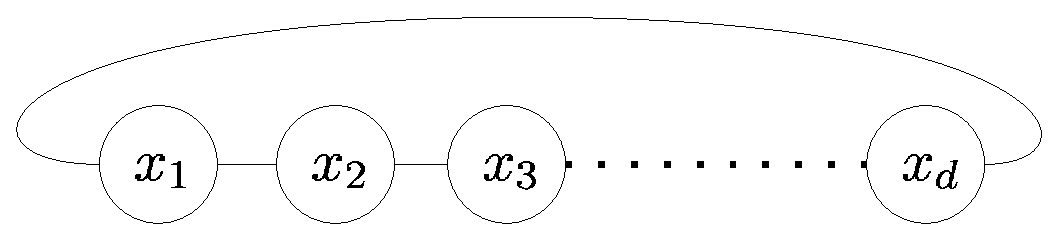
\includegraphics[width=\hfiglength\linewidth]{data_etc/1d_ising.eps}}
\caption{1D Ising with Periodic Boundary Conditions.}
\label{fig-1d}
\vspace{0.2in}
\centerline{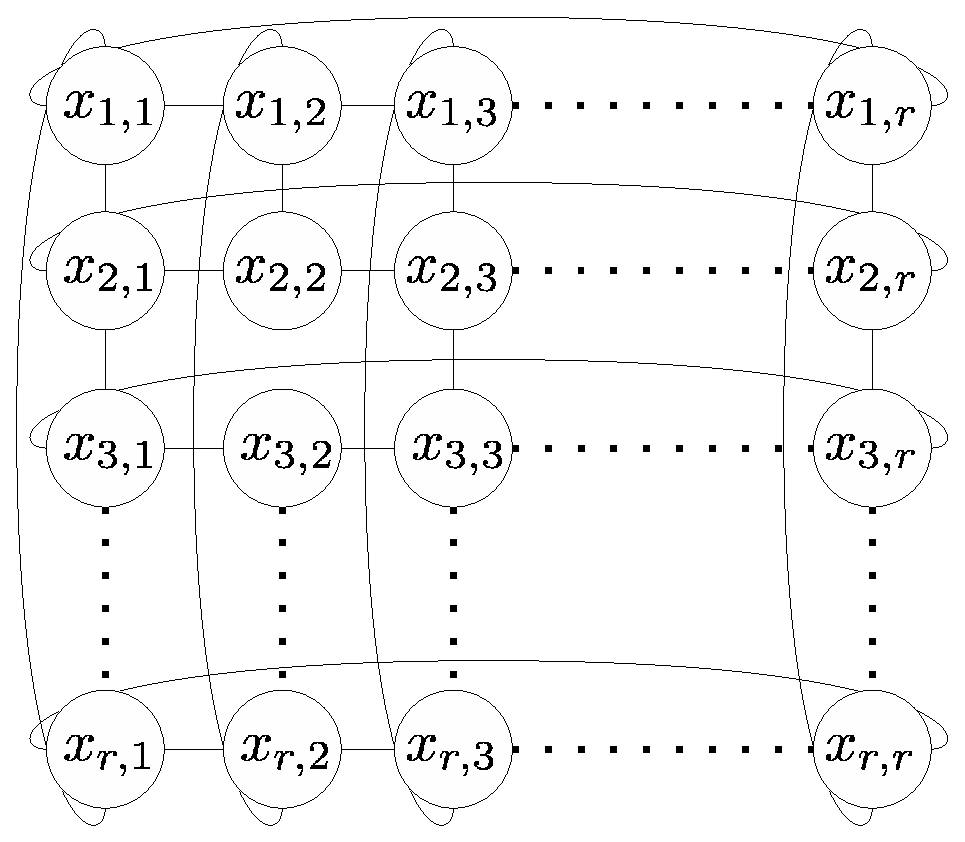
\includegraphics[width=\hfiglength\linewidth]{data_etc/2d_ising.eps}}
\caption{2D Ising with Periodic Boundary Conditions.}
\label{fig-2d}
\end{figure}


\subsubsection{Adding Noise}
Since the threshold of the partially uniform distribution
cannot function precisely
when multiple solutions have the same cost function value,
the original cost function $f(x)$ is slightly altered
by adding small random values $\epsilon$ as follows:
\begin{equation}
 f'(x)=f(x)+\epsilon
.
\end{equation}
In the experiments,
$\epsilon$ is $u \times 10^{-10}$, where $u$ is a random number
uniformly distributed from $0$ to $1$.
This is applied to all the three functions described above.



\subsection{Experimental Setup}
\label{exp-rpm-setup}
This thesis focuses on the simplest probability model, 
that is, a fully factorized one defined as follows:
\begin{equation}
 p(x|w)=\prod_{i=0}^{i=d-1} p(x_i|w_i),
\end{equation}
where each $p(x_i|w_i)$ is a Bernoulli distribution.
This is because, for the first step in investigating the effects of HIS,
the basic probability model is appropriate 
in terms of avoiding over-fitting.
Instead of changing the complexity of the probability models,
different kinds of problems are used for the experiments.
As future work, investigations on the effects of model errors on HIS 
will be performed 
by changing the complexity of the probability models.

When using the factorized probability model, 
FR (EDA) corresponds to UMDA \cite{muhlenbein:umda}.
Probability models are built by using ML estimation.
Only in the cases of FR,
we employ online updating where
the parameter is updated by
\begin{equation}
 w_{new}=(1-\alpha) w_{old} + \alpha w_{ML},
\end{equation}
where $w_{new},w_{old},w_{ML}$ are the new parameter,
previous parameter, and ML estimator, respectively, and
$\alpha$ is the learning rate.
This is because the population is quickly changed in FR and 
this causes instability. In the present experiments, $\alpha=0.5$.


In all cases, there are basically three parameters:
(1) the population size, denoted by $N$,
(2) the number of generated samples in one sampling, denoted by $M$, and
(3) cutoff rate, denoted by $c$.
These values are experimentally determined as follows:
{
\begin{itemize}
\item FR (EDA)
\begin{itemize}
\item $N$: $100$, $500$, $1000$, $3000$, or $6000$.
\item $M=N$.
\item $c$: $0.1$, $0.3$, or $0.5$.
\end{itemize}
\item ER
\begin{itemize}
\item $N$: $100$, $500$, $1000$, or $3000$.
\item $M=N \times c$.
\item $c$: $0.1$, $0.3$, $0.5$, or $0.7$.
\end{itemize}
\item RTR
\begin{itemize}
\item $N$: $10$, $50$, $100$, $200$, $300$, $400$, or $500$.
\item $M(\leq N)$: $10$, $50$, $100$, $200$, $300$, $400$, or $500$.
\item $c$: $0.1$, $0.3$, $0.5$, $0.7$, or $0.9$.
\end{itemize}
\item RPM
\begin{itemize}
\item $N$: $10$, $50$, $100$, $200$, $300$, $400$, or $500$.
\item $M(\leq N)$: $10$, $50$, $100$, $200$, $300$, $400$, or $500$.
\item $c$: $0.01$, $0.05$, $0.1$, or $0.2$.
\end{itemize}
\end{itemize}
}
The stopping criteria are that the number of function evaluations
is greater than $2.9\times10^6$, 
the variance of the cost function values
of the generated samples is less than $10^{-20}$,
and the optimal solution is found.


\subsection{Results}
\newcommand{\ersfigure}[2]{\begin{figure}[t]
\begin{center}
\begin{tabular}{p{\hfiglength\linewidth}p{\hfiglength\linewidth}}
\begin{minipage}{\linewidth}
\centerline{\includegraphics[width=\linewidth]{./data_ers/#2.eps}}
\end{minipage}
&
\begin{minipage}{\linewidth}
\centerline{\includegraphics[width=\linewidth]{./data_ers/#2_var.eps}}
\end{minipage}
\\
\spcen
(a) Entropy
&
\spcen
(b) Standard Deviation
\\
\end{tabular}
\vskip -0.2in
\caption{#1}
\label{figers-#2}
\end{center}
\end{figure}
}

\ersfigure{A typical evolution for onemax in using partially uniform distributions.}{t_ers_0d}
\ersfigure{A typical evolution for 1D Ising in using partially uniform distributions.}{t_ers_1d}
\ersfigure{A typical evolution for 2D Ising in using partially  distributions.}{t_ers_2d}
\ersfigure{A typical evolution for onemax in using Boltzmann distributions.}{ers_0d}
\ersfigure{A typical evolution for 1D Ising in using Boltzmann distributions.}{ers_1d}
\ersfigure{A typical evolution for 2D Ising in using Boltzmann distributions.}{ers_2d}

The results of FR (EDA) are shown in Appendix \ref{exp-edace}.
A part of the results for onemax are shown in Tables \ref{result_0d_idea}
, \ref{result_0d_rtr} and \ref{result_0d_rpm}.
The columns titled ``Best'' list 
the average cost function values, with the standard deviation in parenthesis,
of the best obtained solutions over ten independent runs.
The columns titled ``Evaluations'' 
list the average number, 
with the standard deviation in parenthesis, 
of function evaluations performed  until stopping criteria are met.
The others show the parameters.
Basically, FR, ER and RPM afford sufficient good results,
that is, finding an optimal solution.
In contrast, in some RTR cases,
the population does not converge and
the obtained solutions are bad. 
The results imply that
RTR needs appropriate parameter setting especially on
the cutoff rate, though
it may be difficult to select an appropriate parameter in general.
RTR with $c=0.7$ is comparatively good for onemax.

The results for 1D and 2D Ising are shown in 
Figs. \ref{result_1d} and \ref{result_2d}, respectively.
In each figure,
the horizontal axis represents the number of function evaluations,
while the vertical axis represents the cost function value.
Each point represents the average cost function value of the best obtained
solutions and the average number of function evaluations performed
over ten independent runs for FR, ER and RPM.
Note that RPM with $C=0.1$ and $C=0.2$ are not shown
because in these cases the population quickly converges
and the results are not good.
The results of these cases with $M=500$ are shown in
 Fig. \ref{result_cutoff}.
In RTR, the population does not converge and therefore
the average cost function value of the best case is represented by 
the horizontal line in each figure.
The five best cases of RTR for 1D and 2D Ising are shown in 
Tables \ref{table_rtr_1d_2d}-(a) and \ref{table_rtr_1d_2d}-(b), respectively.
For comparison,
a part of results of RPM are also shown in tables
\ref{table_rpm_1d_2d}-(a) and \ref{table_rpm_1d_2d}-(b).
The expression is the same as in the previous tables. 

As shown in the results for 1D and 2D Ising,
if sufficient number of function evaluations 
are performed until convergence
RPM is clearly the best method.
ER may be slightly better than FR.
RTR can afford better solutions than ER,
but RTR has the problem of convergence
and may have the difficulty in parameter setting,
It is pointed that
RTR with tournament selection is better than
RTR with truncation selection in \cite{lima:replacement}.


\section{Discussion}
\subsection{Diversity of Population}
The quality of a population depends on both 
the average of the cost function value over the samples in the population
and
the diversity of the population.
If we keep only samples with better cost function values,
the population will quickly converge into local optima.
To prevent this, it is important to
search promising area
where samples have not been generated yet,
by keeping the diversity.

In RPM, 
the diversity is kept not by resampling, but by weighting
\footnote{ It is clearly optimal that no samples are removed.
Even in this case, the diversity can be controlled by weighting.
The role of resampling is to keep the population size constant.}.
In calculating the empirical log-likelihood,
small weight samples are basically ignored or removed.
The weights are defined by (\ref{weight-update}).
In (\ref{weight-update})
samples with higher value of $p(x)$ have smaller weight.
This means that
samples in an area where many samples are generated, 
are regarded as less important.

To generate samples from the target distribution $q(x)$ 
is supposed to be the optimal in the EAPM framework.
However, in practice, the samples are generated from 
a probability model $p(x)$ approximating $q(x)$
and the samples have a bias because
$p(x)$ is a simple function whereas $q(x)$ is a complex function in general.
Then, the role of (\ref{weight-update}) is
the correction of the sampling bias of $p(x)$.

CE actually has this bias removing mechanism 
but cannot afford good results.
This is because generated samples are unstable
due to the estimation error of $p(x)$ in approximating $q(x)$.
In contrast, the population in RPM theoretically does not
depend on $p(x)$ and consequently RPM affords good results. 
This implies that the population mechanism of RPM
improves the quality of samples in calculating the empirical
log-likelihood, where samples from $p(x)$ may be bad.


\subsection{Control of Convergence Speed}
In RPM, the convergence speed is controlled by
the target distribution, that is, 
the threshold parameter of partially uniform distribution.
It is guaranteed that
the threshold is monotonically decreased in RPM and
the population must converge eventually.
ER possesses the similar property.

The convergence speed has an effect on the
accuracy of importance sampling of (\ref{eapm-ml}).
To generate samples from the current target distribution is
the optimal case.
In this case, the weight is defined by $\frac{q_{t+1}(x)}{q_t(x)}$.
If $q_{t+1}(x)$ and $q_t(x)$ are similar, the accuracy of importance
sampling becomes better.
In other words, slow convergence improves the accuracy and
helps to afford good results.
Through the experiments,
it is confirmed that 
RPM is actually the only method that can monotonically control
its convergence speed by the cutoff rate as shown in Fig. \ref{result_cutoff}.


\section{Summary}
This chapter proposed Resampling Population Model (RPM),
where a part of the historical samples are stored as the population
to follow the target distribution
from the viewpoint of importance sampling.
Experimental comparisons between RPM and the
conventional population mechanisms have revealed
the following two advantages of RPM: 
(1) RPM affords better solutions than the conventional methods and 
(2) RPM can monotonically control the convergence speed by using the
cutoff rate.







